\frame
{
\begin{center}
	\Huge{Técnicas}\\
	\huge{Hierarchical Shotgun Sequencing}
\end{center}
}

\frame
{
\frametitle{Hierarchical Shotgun Sequencing}
\framesubtitle{¿Qué es?}
\begin{itemize}
	\item También conocida como técnica del \emph{``clon-por-clon''}
	\item Es el método \red{preferido} por el Proyecto del Genoma Humano.
	\item Por lo general es utilizado en genomas con \blue{repeticiones}.
	\item Es \blue{recomendable} utilizar en Eucariontes en general.
	\item Utiliza enzimas en su proceso.
\end{itemize}
}


\frame
{
\frametitle{Hierarchical Shotgun Sequencing}
\framesubtitle{Ventajas y Desventajas}
\begin{itemize}
	\item \blue{Ventajas:}
	\begin{itemize}
		\item Detecta secuencias repetidas.
		\item No tiene problemas de regiones poco representadas.
	\end{itemize}
	\item \red{Desventajas:}
	\begin{itemize}
		\item Demora mucho tiempo.
		\item Posee mucho costo computacional.
	\end{itemize}
\end{itemize}
}


\frame
{
\frametitle{Hierarchical Shotgun Sequencing}
\framesubtitle{¿Cómo funciona?}
\begin{enumerate}
	\item<1-> Construir una \blue{genoteca} por fragmentación del ADN (utilizando BACs)
	\begin{itemize}
		\item<1-> BAC : Bacterial Artificial Chromosomes.
	\end{itemize}
	\item<2-> Los fragmentos de ADN representados en la misma son organizados en un \blue{mapa físico}.
	\item<3-> Elección al azar de colonias y se \blue{replican}.
	\item<4-> Los clones individuales son \blue{seleccionados al azar} y secuenciados.
	\item<5-> Para el paso anterior es necesario hacer una \blue{nueva genoteca} de trozos más pequeños
	\item<6-> La secuencia de los clones se \red{ensambla finalmente} para reconstruir la secuencia del genoma.
\end{enumerate}
}
%Proceso:
%    DNA target (muchas copias)
%        Enzima de restriccion de baja frecuencia de corte.
%        fragmentos de 10 a 1000kb
%    YACS (Yeast artificial chromosome)
%    Mapeo fisico
%    Eleccion al azar de algunas colonias
%    Se replican
%    Se elige un clon
%        Enzima de restricciones de alta frecuencia
%        fragmentos cortos (40kb)
%    Inclusion de fragmentos en cosmidos
%    Introduccion de fragmentos en bacterias
%    Secuenciacion de fragmentos pequeños
%
%    Ensamblado de secuencias de fragmentos cortos.

\frame
{
\frametitle{Hierarchical Shotgun Sequencing}
\framesubtitle{¿Cómo funciona?}
\begin{center}
	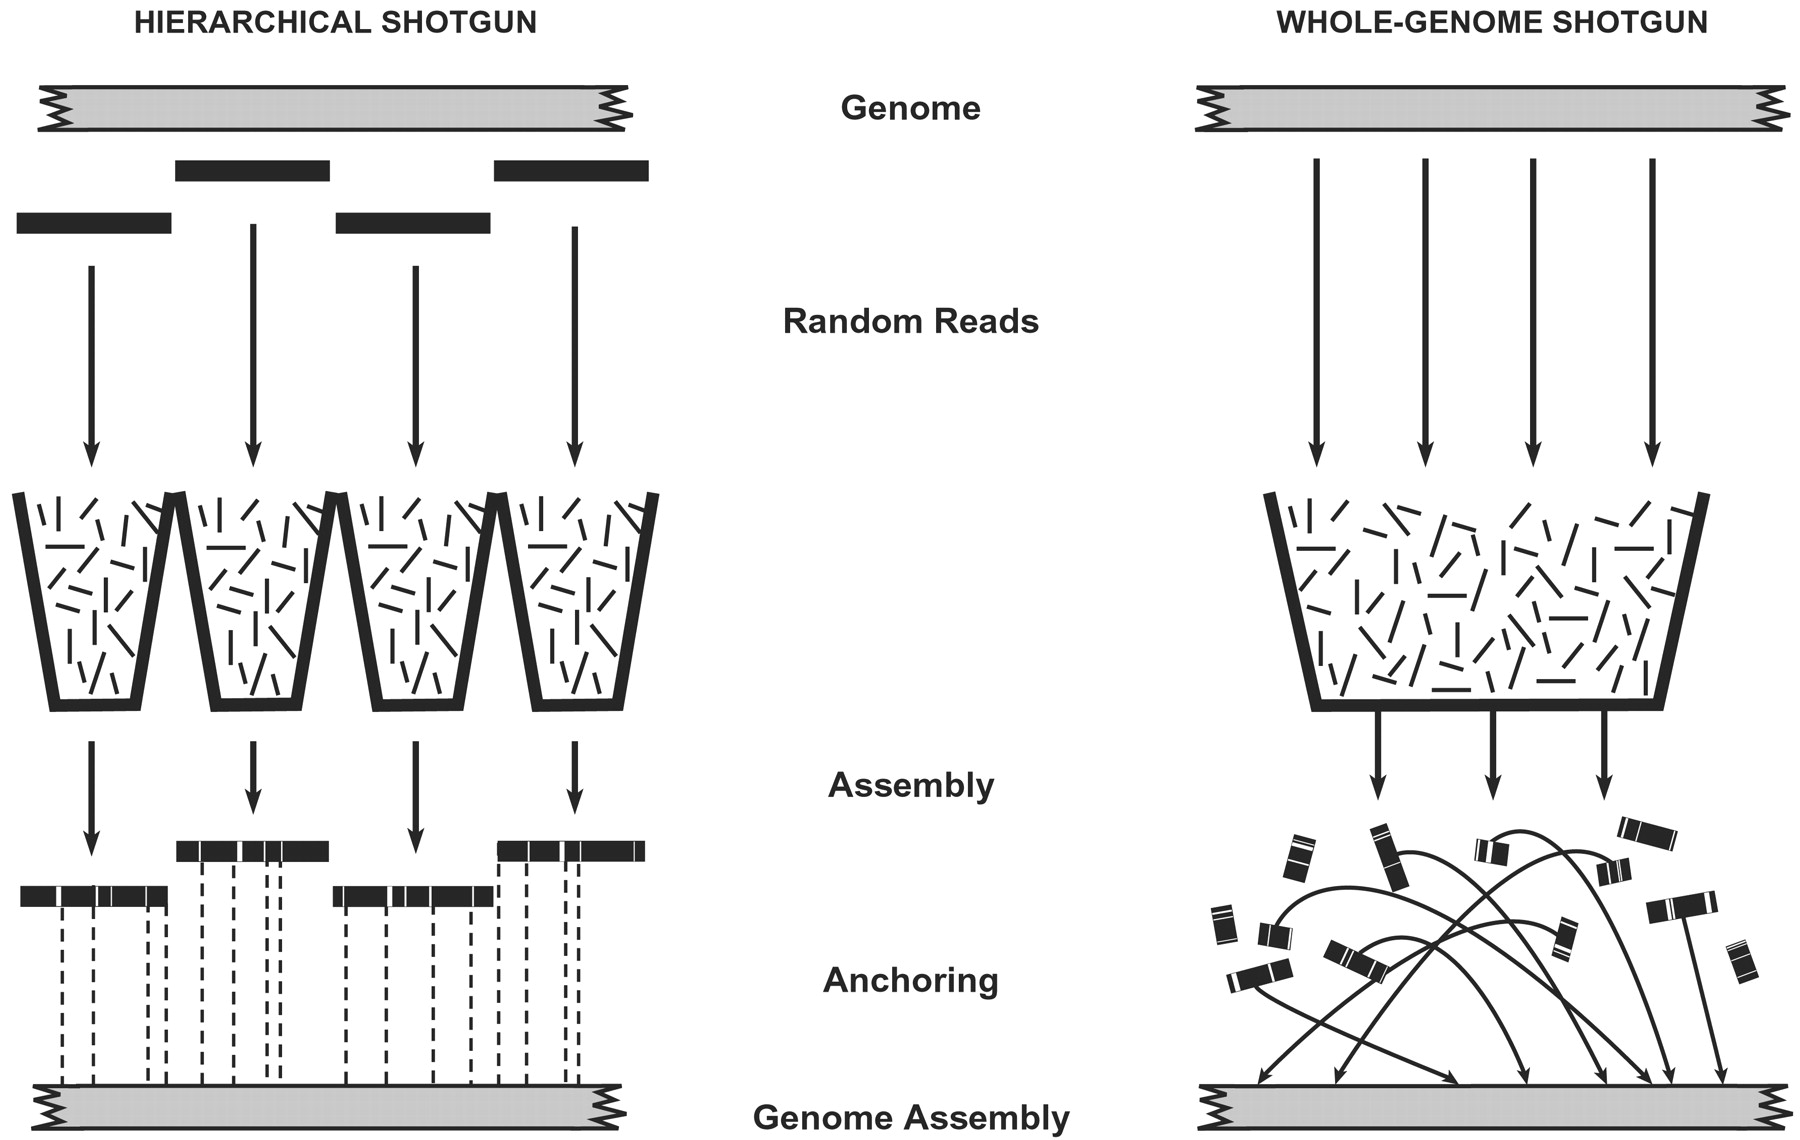
\includegraphics[width=0.9\textwidth]{img/shotguns}
\end{center}
}

\frame
{
\frametitle{Hierarchical Shotgun Sequencing}
\begin{center}
	\huge{Video}
\end{center}
}
